\chapter{Background}
This section presents the 
this is short and needs a lot more detail and also figures.

This section briefly reviews the current techniques for lung perfusion and hemodynamic
monitoring, and provides a general overview 
of the state of 3D EIT as used for thoracic imaging and monitoring.


\section{Impedance Imaging}
\label{sec:impedance_imaging}
Impedance imaging has been in use since the early 1900s for geophisical applications.  
Originally introduced as a technique to image below the earth’s surface, 
current was transmitted between two electrodes placed into the ground and any 
anomalies in subsurface conductivity produced deviation 
in the equipotential lines. 
Including current injections and measurements from multiple locations and using known 
electrical properties of geological structures Conrad Schlumberger identified
features of underground geological structures~\parencite{allaud_schlumberger_1977}.

These same techniques can be applied in biomedical applications where
voltage is measured on an array of body surface electrodes 
while current is applied between select electrode pairs (\fref{fig:cur_equip_line}). 
Due to impedance differences associated with biological tissues and their physiological 
function~\parencite{geddes_specific_1967,mcadams_tissue_1995},
EIT has been proposed for a wide range of applications from thoracic monitoring
\parencite{frerichs_chest_2017} to neuronal and 
brain imaging~\parencite{holder_electrical_1992}.

\begin{figure}
    \centering
   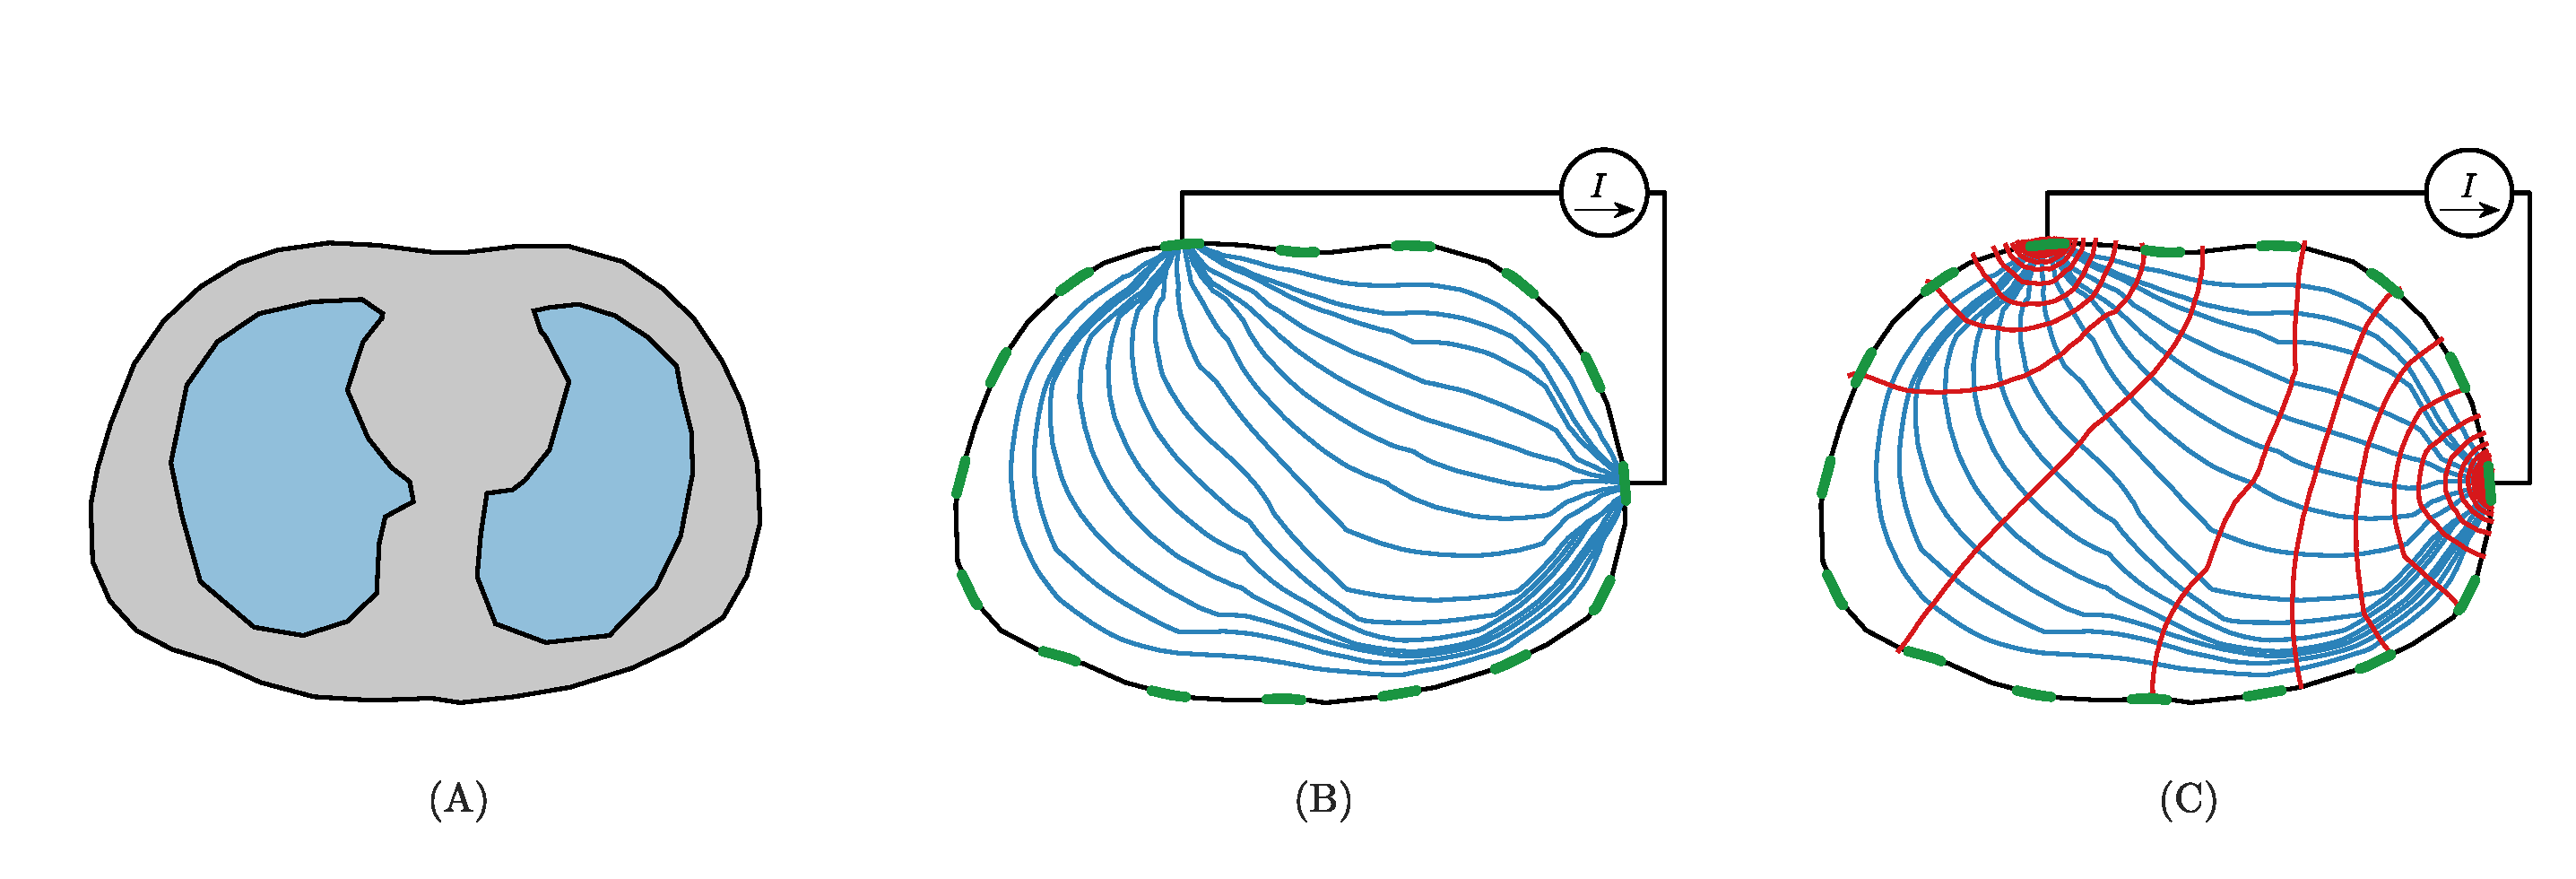
\includegraphics[width=\textwidth]{chapter2-background/imgs/current_and_equipotential_lines.pdf}
   \caption[Current and Equipotential lines]{\label{fig:cur_equip_line} 
   (A) A body comprising tissues of different conductivity, (B) Electrodes are placed on the surface 
   and current is injected between a pair or electrodes. The current pathways are indicated 
   by the blue lines. (C) The resulting equipotential lines within the body are shown in red.}
\end{figure}

\section{Bioimpedance}
\label{sec:bioimpedance}
In thoracic imaging the most commonly measured 
impedance changes occur due to movement 
of air in the lungs, the flow of blood, and the motion of 
organs~\parencite{adler_electrical_2017}. 
During inhalation, the volume of air in the lungs increases, lowering the 
conductivity of the lung tissue. 
The resistivity of lung tissue varies significantly
between expiration and inspiration giving a value of 7 $\Omega$ m during expiration
and 23 $\Omega$ m during inspiration at 100 kHz~\parencite{witsoe_electrical_1967},
resulting in a
measureable variation in impednace during respiration~\parencite{eyuboglu_vivo_1989}. 
There are also other 
signifant sources of impedance change that make EIT signal intrepretation 
challenging. Simulations have attributed up to 20
percent of the respiratory signal to the effect of 
chest expansion and movement of the chest 
wall~\parencite{adler_impedance_1994}.

The source of impedance changes due to the flow of blood is even more complex. 
Since the resistivity of blood is so much lower than other tissues 
(1.5 $\Omega$ m), the increase of blood due to pulsatile 
flow should decrease the impecance of structures it passes through 
by a detectable amount~\parencite{eyuboglu_vivo_1989}.
It is often assumed that the component of EIT images at the cardiac 
frequency is related to the perfusion of blood, but the exact source of
cardiosynchronus EIT signals is 
unclear~\parencite{patterson_impedance_2010,nguyen_review_2012}.
A continuous flow of blood alone is insufficient 
to induce a significant impednce change, 
as the volume and concentration of the conductive medium is unchanged. 
Any impedance-based measure of perfusion relies on the cardiosynchronous 
EIT signals which have numerous possible sources~\parencite{adler_origins_2017}. 

\subsection{The Cardiac Cycle}
%The following subsection is a brief overview on elements of 
%the cardiac cycle that
%relate to perfusion imaging with EIT.
The cardiac cycle consists of the activity in the heart between the
beginning of one heart beat, and the next. There are two main stages 
of the cardiac cycle: the diastole, when the heart relaxes and is filled 
with blood, and the systole, when contraction of the heart pumps blood to
lungs and all other body systems~\parencite{pappano_cardiovascular_2019}. 
A simplified anatomy of the heart is 
presented in \fref{fig:anatomical_heart}. 
Since ECG recordings are frequently used to synchronize 
EIT data, it is helpful to look at the timing of the cardiac cycle as it 
relates to features of ECG traces. An example ECG waveform is pictured in 
\fref{fig:cardiac_bioimpedance}. 

\begin{figure}
    \centering
    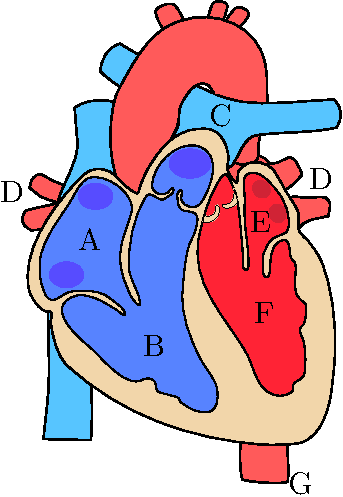
\includegraphics[width=0.6\textwidth]{chapter2-background/imgs/heart_drawing.pdf}
    \caption[Sketch of the anatomical heart]{ The pathway of the blood
    from entry to the heart to the descending aorta is indicated by the
    letters. Deoxygenated blood enters the heart through the right atrium
    (A) where it is moved to the right ventricle (B). From there it passes through 
    the pulmonary artery (C) into the lungs where it perfuses and is oxygenated. 
    Blood return from the lungs through the pulmonary veins (D) then enters 
    the left atrium (E). Finally, the blood is pumped from the left
    ventricle (F) to the rest of the body through the aorta, and the
    descending aorta (G).}
    \label{fig:anatomical_heart}
\end{figure}

During the first stage of the cardiac cycle is the ventricular
diastole, indicated by the P wave on an ECG trace, during 
which the heart relaxes and expands
pulling blood into the ventricles from the 
atria~\parencite{pappano_cardiovascular_2019}. Blood enters the atrium 
on the right side of the heart through the
superior and inferior vena cava and on the left side of the heart, the atrium is 
filled by oxygenated blood from the lungs through the pulmonary 
veins~\parencite{pappano_cardiovascular_2019}.
Next is the atrial contraction during which time the atria pump additional
blood into the ventricles, and the ventricular volume and pressure 
is maximized. At the peak of the ventricular volume, the ventricles contract 
and depolarize which corresponds to the QRS complex~\parencite{pollock_physiology_2021}. 
On the right side of the heart, deoxygenated blood is pumped 
to the lungs where it perfuses into the lung tissue, and on the left side of 
the heart oxygenated blood is pumped to the rest of the body through the 
aorta~\parencite{pappano_cardiovascular_2019}. The smallest volume in the ventricles occurs after 
the ventricular repolarization represented in the ECG by
T wave~\parencite{pollock_physiology_2021}.

\begin{figure}
\centering
\begin{tikzpicture}[line join=round, x=2pt, y=-2pt]
    \tikzset{
        normal ecg/.pic={
            \draw (0,455.0021) -- (11.8345,455.0021);
            \draw (11.8345,455.0021) .. controls (14.2834,454.8958) and
                (14.1385,448.7114) .. (18.8842,448.7114) .. controls (24.2116,448.7114) and
                (23.9695,454.8958) .. (26.3035,455.0021) node[above, xshift=-22pt, yshift=21pt] {P};
            \draw (26.3035,455.0021) -- (40.7723,455.0021) node[below, xshift=5pt, yshift=-25pt] {Q} ;
            \draw (40.7723,455.0021) -- (42.7455,463.0645) -- (46.0339,413.3461) node[above, xshift=0pt, yshift=0pt] {R}
                -- (48.6647,466.4235) -- (51.2955,455.0021) node[below, xshift=-7pt, yshift=-35pt ] {S} ;
            \draw (51.2955,455.0021) -- (61.1605,455.0021);
            \draw (61.1605,455.0021) .. controls (64.4487,454.3298) and
                (65.7118,441.6860) .. (70.3679,441.5241) .. controls (75.2428,441.3542) and
                (76.9447,454.3301) .. (80.2329,455.0021) node[above, xshift=-29pt, yshift=39pt] {T};
            \draw  (80.2329,455.0021) .. controls (81.4852,455.0021) and
                (82.2677,452.8462) .. (84.1792,452.9863) .. controls (85.8717,453.1101) and
                (86.4830,455.0021) .. (87.4678,455.0021); % node[above, xshift=-10pt, yshift=5pt] {U};
            \draw (87.4678,455.0021) -- (100,455.0021);
        }
    }
    \foreach \x in {0}{
    \pic [very thick, scale=1.5] at (\x*50, 0) {normal ecg};
    }
\end{tikzpicture}
\caption[Example ECG waveform]{ An example ECG waveform to compare electrical signals in the 
heart to blood volume changes.
The P wave represents the beginning of the cardiac cycle with the ventricles begin to fill. The QRS complex
corresponds with ventricular depolarization 
and occurs as the ventricles contract they contract.  The beginning of the QRS complex corresponds with 
the maximum ventricular volume. The minimum 
volume in the ventricles occurs after ventricular repolarization represented by the T wave.}
\label{fig:cardiac_bioimpedance}
\end{figure}

\subsection{Bioimpedance of Perfusion} \label{sec:origins}
There are several factors that may contribute some part of 
the impedance change during the cardiac cycle. 
Some of these factors include:
\begin{itemize}
    \item Changes in blood volume within the heart as blood is pumped. As the ventricles 
          fill with blood
          the volume increases and results in a more conductive
          heart~\parencite{nyboer_impedance_1970}.
    \item Variations in arterial and blood vessel volume. Due to the elasticity of arteries 
          and
          blood vessels, the pulsatile flow of blood passing through results in variation of 
          vessel diameter, affecting the impedance~\parencite{eyuboglu_localisation_1987}.
    \item Physical deformation of structures due to motion of the heart. The
          motion of the heart can have significant contribution 
          to cardiosynchronous EIT 
          images~\parencite{proenca_influence_2015,adler_origins_2017}, 
          with simulations showing that heart motion was the 
          main contributor to impedance change due to the 
          ventricle~\parencite{proenca_influence_2015}. 
    \item The orientation of red blood cells. During pulsatile flow the orientation of
          red blood cells changes, which had been shown to affect the impedance of the 
          blood~\parencite{gaw_effect_2010}. 
    \item Ballistic forces in the body generated by the heart. During each
          heartbeat blood is pumped downwards through the descending
          aorta with a large force pushing the rest of the body 
          upwards~\parencite{gordon_certain_1877}. Different directions 
          of flow in the aorta result in a repeating ballistic 
          signal on the rest of the body~\parencite{kim_ballistocardiogram_2016}. This results in 
          motion on the electrodes and body which can introduce significant
          artefacts in EIT signals~\parencite{adler_impedance_1994}.
\end{itemize}

The contribution of each of these factors will ultimately depend on the placement
of the electrodes and the specific geometry and physiology of a patient. 
When imaging changes in stroke volume, changes 
relating to posture, breathing and changes in belt 
position resulted in  changes that overpowers the 
perfusion signals~\parencite{patterson_variability_2001}.  

Despite the challenges of isolating cardiosynchronous EIT signals related to 
perfusion there is still a great interest in 
improving accuracy and stability due to the unique 
advantages offered by EIT over current state-of-the-art methods.

\section{Perfusion Imaging}

Determining the flow of blod within vital organs such as the heart, brain and lungs 
allows doctors to make quivk dicieiosn to treat patients in life threatning situations.
In the braing perfusion imaging can be used to diagnose and monitoor dementia
and Alzheimer's disease \parencite{dougall_systematic_2004,barker_pathophysiology_2014},
or to detect and diagnose ischemic strokes 
\parencite{koenig_perfusion_1998,konstas_theoretic_2009}. 
Perfusion images of the heart can be used to diagnose ischemic 
heart disease \parencite{prvulovich_role_1998}, which is caused by a reduction 
of blood flow to the heart, typically due to 
a build-up of plaque in the arteris of the heart
\parencite{mendis_global_2011}. Ventilation/perfusion scans can be used in the 
lungs to measure the distribution of perfusion and ventilation in the lungs 
\parencite{mortensen_lung_2019}. The primary use 
is to detect mismatches between the ventilation in perfusion to detect pulmonay 
embolysms \parencite{pioped-investigators_value_1990}.   

Nuclear medicine has been at the forefrtont of perufsion imaging, but has a long
acquisition time, and images can be fuzzy and challenging to intrepret \parencite{prvulovich_role_1998}. 
Recent developments in \acrfull{ct} and magnetic resonance imaging \acrshort{mri} 
imaging yeild clearer images and can give metrics 
regarding blood flow and blood volume over a period of 
time \parencite{prvulovich_role_1998}. 
EIT has been proposed as a technique to monitor perfusion due 
to its sensitivity to blood movment, 
and development is currently underway to 
establish EIT as a technique to monitor 
perfusion \parencite{nguyen_review_2012,nguyen_perfusion_2015}, 
blood flow \parencite{braun_limitations_2018,braun_accuracy_2018}, and 
blood pressure \parencite{proenca_noninvasive_2017,proenca_non-invasive_2020}. 
The following section 
explores the advantages and pitfalls of state of the art perfusion monitoring techniques. 


\subsection{Nuclear Medical Imagaing}
The two primary nuclear medicine techniques used for perfusion imagaing are 
single-photon emission computed tomography (\acrshort{spect}), and scrintigraphy. 
These techniques image gamma rays that are emitted from a gamma-emitting radionuclidite
injected into the patient \parencite{mettler_essentials_2006}. 
The radioisotopes are integrated into drugs 
that enable them to travel to a specific organ or tissue. 
Perfusion imaging with scintigraphy and SPECT 
is primarily used in the lungs and heart. 
The emitted gamma rays are measured by external detectors called 
gamma cameras \parencite{mettler_essentials_2006}. 
The main difference between the two is that SPECT creates 3D images, and 
scintigraphy images are 2D.
Scintigraphy uses a gamma camera place in a single location, while SPECT 
uses a detector that roates around the patient and captures gamma images from 
several angles. A typical SPECT system rotates 3--5 degrees per acquisiton 
and takes apprximately 15--20 minutes to complete a full scan,
although scan times can be shorter when multiple detectors are used to capture
images from multiple angles simultaneously \parencite{mettler_essentials_2006}.

Nuclear medical imaging can be used to image both ventilation and perfusion which 
has been used to diagnose pulmonary embolysms \parencite{mortensen_lung_2019}.
Ventilation/perfusiuon scans area a specefic type of perfusion scan that uses lung
scintigraphy. During ventilation an aresolized radionuclitide is inhaled through a mask placed
over the nose and mouth. To image lung perfusion a different radionuclitide 
is injected and its passage through 
the lung is imaged.
Both phases are imaged using a gamma camera \parencite{mortensen_lung_2019}. 
This technique can be time and labour intensive, and results in 
radiation exposure to both the technitian and patient \parencite{gandev_comparison_2005}.
The duration of a single scan to measure ventilation and  
perfusion is approximately 15 minutes, including time time required to breath the radionuclidite
prior to imaging \parencite{hur_optimizing_2014}. Reducing the time 
required to imrove image acquisition time and reduce radiation exposure
has been shown to give less reliable measures of perfusion \parencite{hur_optimizing_2014}.
Nuclear medicine imaging methods have a lower radiation dose than CT perfusion imaging techniques,
but suffer from a much lower resolution and lunger imaging time \parencite{aljizeeri_ct_2013}. 
As such CT is becoming the prefered 
method to image myocardial perfusion \parencite{aljizeeri_ct_2013}. 

\subsection{CT}

Contrast-enhanced CT has been used since 1980 to estimate perfusion in the brain 
and estimate perfusion \parencite{axel_cerebral_1980}. Contrast enhanced perfusion imagang 
has been used to image perfusion due to ischemic stroke 
\parencite{miles_colour_1991,koenig_perfusion_1998}.
This teqhnique uses an injection of 25--35 mL 
of a constrast agent, and the progress of the constrast agent through blood vessles 
and capillaries near to the brain is imaged over  75--90 seconds. Techniques are typically used to reduce overall 
radiation exposure, but imaging duration is limited by safety concerns due to radiation exposure
\parencite{konstas_theoretic_2009}.
Constrast-enhanced CT has also been found to be an effective and cost effective 
technique to image myocardial perfusion in cardiovascular disease
\parencite{aljizeeri_ct_2013}, but images require an invasive cardiac catheterization and 
pose a risk of radiation exposure to 
both patients and technitians \parencite{vijayalakshmi_cardiac_2007}.

\subsection{MRI}

There are three main techniques used to image perfusion using 
MRI. The first uses a contrast agent to image wich is used to either induce a reduction of 
amplitude in %T2*-weighted 
images \parencite{jackson_dynamic_2005} the concentration of 
contrast agent present in the images can be used as an approximation of 
perfusion \parencite{jackson_dynamic_2005}. 
The second technique also uses an injected contrast
agent. This technique images the transit of a contrast agent as it travels 
from the blood into a tissue \parencite{sourbron_classic_2013}. In this technique the contrast
agent is not imaged directly, but impacts the magnetic properties of 
water molucles it passes resulting in a change in image intensity in regions 
with constrast agent \parencite{sourbron_classic_2013}. 
The final technique is atretical spin labelling, which does not rely on 
an injected constrasat agent, but rather applies a  magnetic label to the water 
in blood and the perfusion is estimated be tracing the flow of this labelled 
blood \parencite{koretsky_early_2012}. 

MRI is typically used for cerebral perfusion imaging due to its safety and 
lack of ionozing radiation \parencite{watson_lessons_2015}. It is not suitable for 
continuous perfusion imaging due to the acquisiton time which which 
ranges from 1-5 minutes depending on the method \parencite{essig_perfusion_2013},
and it can not be used at the bedside.

\subsection{EIT}
EIT has been suggested as an ideal tool to continuously monitor 
perfusion \parencite{leonhardt_electrical_2012}. EIT is cost-effective,
non-invasive, does not use ionizing radiation, and images can be acquired 
contiunuoisly at a high sampleing rate \parencite{adler_electrical_2017}.
Despite these advantages of EIT, 
spatial resolution is low, and image accuracy is further limited by 
artefacts introducted by poor electrode contact and electrode 
movement \parencite{adler_electrical_2017}.
The spatial resolution of EIT is typically thought to be approximately 20--50\% 
of the electrode seperation, but can be afectetd by the measurement protocol 
and image reconstruction techniques \parencite{polydorides_electrode_2002}.

EIT has been evaluated for its ability to measure cardiac output and
lung perfusion since the late 1980s
\parencite{eyuboglu_vivo_1989,zadehkoochak_pulmonary_1992,brown_blood_1992,frerichs_regional_2002}.
Since then, various configurations of EIT have been 
evaluated~\parencite{borges_regional_2012,nguyen_perfusion_2015}.
Due to the speed and safety of measurement acquisition, EIT might be used to continuously monitor 
perfusion in subjects mush more frequently than current state of the art techniques.

There are two main ways perfusion related changes can be imaged with EIT. Like with many 
perfusion imaging techniques, a contrast agent can be injected to image the transit 
of blood through vessels and organs.
Typically a sodium chloride bolus with a concentration between 
5--20\% is used as a contrast agent for EIT \parencite{nguyen_review_2012}, 
and an algorithm to determine the regional blood flow to the lung and heart
\parencite{borges_regional_2012}. This technique was found that measures of perfusion 
using a contrast agent with EIT were highly correlated to SPECT images of perfusion
\parencite{borges_regional_2012}.
The same study found that pulsatile images of EIT showed little correlation to bolus measures 
and SPECT scans. 

When breathing is paused, the signals based only on 
the cardiac activity can be more easily extracted. 
It was found that during apnoea the global impedance 
recorded with EIT measurements corresponded with stroke volume 
measured using the 
thermodilution method with a pulmonary arterial 
catheter~\parencite{fagerberg_electrical_2009}.
Ventilation perfusion ratios have been calculated during apnoea by comparing 
ventilation and perfusion signal amplitude with a specified region of 
interest~\parencite{fagerberg_electrical_2009}.
There is some concern that the perfusion measured 
during apnoea may not accurately represent 
true perfusion during regular respiration as the apnoea 
impacts the regular respiratory cycle~\parencite{leonhardt_electrical_2012}, and since 
apnoea cannot be sustained continuously there is interest in an alternative method 
to increase sensitivity to cardiosynchronous changes. 

The majority of work on perfusion imagingin with EIT has focused on imaging the pulsatile or 
cardiosynchronous component of EIT data \parencite{nguyen_review_2012}. 
As discussed in section \fref{sec:origins} there are many potential sources of 
the cardiosynchronous signal, and the effect of perfusion related changes is not well understood. 
Perfusion had been calculated using digital filtering to extract the related componenet
of an EIT signal. 
\citeauthorandyear{deibele_dynamic_2008} have shown that principal component analysis (PCA) 
can be used to separate ventilation and cardiac frequency signals and identify the component 
related to the heart. Once the cardiac-frequency component of the 
EIT signal is identified the pulmonary component must also be isolated. 
One of the most widely used techniques 
is selecting a region of interest that corresponds 
to the organ, tissue or flow to me measured
\parencite{braun_accuracy_2018,sola_non-invasive_2011}.

Techniques to improve accuracy of EIT models and increase sensitivity 
to cardiosynchronous activity 
such as internal and 3D electrode configurations could improve 
accuracy of techniques to isolate pulsatile
activitiy in a specific region, and could enable an 
improved perfusion measure 
using EIT, and a means of continuously monitoring perfusion during ventilation.
In this thesis we explore the effect of both increased mesh accuracy and internal electrodes,
and discuss their potential for improving sensitivity to perfusion with EIT.
























